\begin{figure}[htbp]
\centering
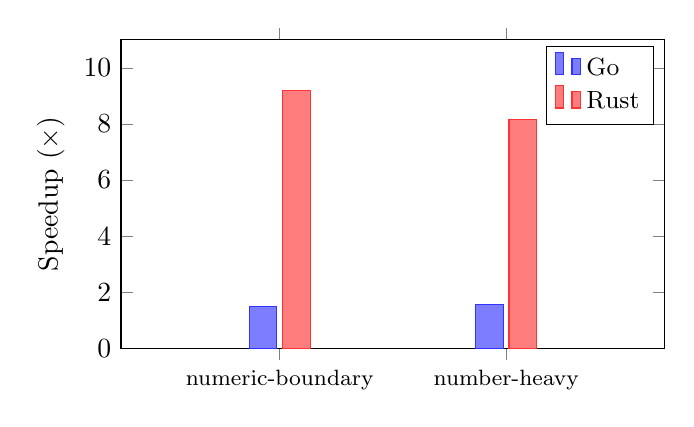
\begin{tikzpicture}
\begin{axis}[
    ybar,
    bar width=10pt,
    width=0.7\columnwidth,
    height=5.5cm,
    ylabel={Speedup ($\times$)},
    xtick={1,2},
    xticklabels={numeric-boundary, number-heavy},
    x tick label style={font=\footnotesize},
    ymin=0,
    ymax=11,
    xmin=0.3, xmax=2.7,
    ytick={0, 2, 4, 6, 8, 10},
    legend style={at={(0.98,0.98)}, anchor=north east, font=\small},
    legend cell align={left},
    every axis plot/.append style={fill opacity=0.85},
]
% Go within-language (schubfach-vs-bd)
\addplot[fill=blue!60, draw=blue!80] coordinates {
    (1, 1.50)
    (2, 1.56)
};
% Rust within-language (schubfach-vs-bd)
\addplot[fill=red!60, draw=red!80] coordinates {
    (1, 9.18)
    (2, 8.17)
};
\legend{Go, Rust}
\end{axis}
\end{tikzpicture}
\caption{API benchmark speedup of fixed-width over \burgerdybvig on the
two pure-numeric workloads ($\nu = 100\%$), shown separately from
Figure~\ref{fig:api-speedup} due to their degenerate number density.
The Go ratios (${\approx}1.5\times$) are consistent with the main
results; the Rust ratios (${\approx}8$--$9\times$) approach
isolation-level speedups because digit generation accounts for
${>}$95\% of pipeline cost on these workloads.  All three fixed-width
algorithms show similar ratios (see text).}
\label{fig:outlier-speedup}
\end{figure}
